% !TeX root = surprises.tex

\chapter{Ein Kompass ist ausreichend}\label{c.compass}

%%%%%%%%%%%%%%%%%%%%%%%%%%%%%%%%%%%%%%%%%%%%%%%%%%%%%%%%%%%%%%%


Lorenzo Mascheroni bewies 1797, dass jede Konstruktion, die mit Lineal und Zirkel ausgeführt wird, auch nur mit einem Zirkel ausgeführt werden kann. Später stellte sich heraus, dass dieses Theorem bereits 1672 von Georg Mohr bewiesen worden war.
Nachdem in Sect.~\ref{s.compass-what} erklärt wurde, was mit der Durchführung einer Konstruktion nur mit einem Zirkel gemeint ist, wird der Beweis in Etappen präsentiert, beginnend mit vier Hilfskonstruktionen: Spiegelung eines Punktes (Sect.~\ref{s.reflection}), Konstruktion eines Kreises mit gegebenem Radius (Sect.~\ref{s.circle}), Addition und Subtraktion von Liniensegmenten (Sect.~\ref{s.add-subtract}) und Konstruktion eines Liniensegments als Verhältnis von Segmenten (Sect.~\ref{s.three}). Abschnitt~\ref{s.two-lines} zeigt, wie man den Schnittpunkt zweier Linien findet und Sect.~\ref{s.line-circle} zeigt, wie man den Schnittpunkt einer Linie und eines Kreises findet.

%%%%%%%%%%%%%%%%%%%%%%%%%%%%%%%%%%%%%%%%%%%%%%%%%%%%%%%%%

\section{Was ist eine Konstruktion nur mit einem Zirkel?}\label{s.compass-what}

Abbildung~\ref{f.compass-equi} zeigt die Konstruktion eines gleichseitigen Dreiecks mit einem Lineal und einem Zirkel. Wie kann man ein Dreieck ohne die Linienabschnitte $\overline{AB}, \overline{AC}, \overline{BC}$ konstruieren? Ein Streckenabschnitt wird durch zwei Punkte definiert, so dass es ausreicht, diese Punkte zu konstruieren, um eine Konstruktion zu erhalten, die derjenigen mit einem Lineal entspricht (Abb.~\ref{f.compass-equi-only}). Es ist nicht notwendig, die Liniensegmente tatsächlich zu sehen.
In den Abbildungen dieses Kapitels wird es Linien geben, aber sie dienen nur dazu, die Konstruktion und den Beweis ihrer Korrektheit zu verstehen. Es ist wichtig, sich davon zu überzeugen, dass die Konstruktion selbst nur einen Zirkel verwendet.
\begin{figure}[ht]
\begin{minipage}{.45\textwidth}
\begin{center}
\begin{tikzpicture}[scale=0.6]
\coordinate (A) at (0,0);
\coordinate (B) at (4,0);
\vertex{A};
\vertex{B};
\draw (A) node[below left] {$A$} -- (B) node[below right] {$B$};
\draw[name path=larc] (A) ++(-10:4cm) arc (-10:80:4cm);
\draw[name path=rarc] (B) ++(-170:4cm) arc (-170:-260:4cm);
\path [name intersections={of=larc and rarc,by={t}}];
\node[above right,xshift=-2pt,yshift=3pt] at (t) {$C$};
\vertex{t};
\draw (A) -- (t);
\draw (B) -- (t);
\end{tikzpicture}
\caption{Konstruktion eines gleichseitigen Dreiecks mit einem Lineal und einem Zirkel}\label{f.compass-equi}
\end{center}
\end{minipage}
\hfill
\begin{minipage}{.45\textwidth}
\begin{center}
\begin{tikzpicture}[scale=0.6]
\coordinate (A) at (0,0);
\coordinate (B) at (4,0);
\vertex{A};
\vertex{B};
\path (A) node[below left] {$A$} -- (B) node[below right] {$B$};
\draw[name path=larc] (A) ++(-10:4cm) arc (-10:80:4cm);
\draw[name path=rarc] (B) ++(-170:4cm) arc (-170:-260:4cm);
\path [name intersections={of=larc and rarc,by={t}}];
\node[above right,xshift=-2pt,yshift=3pt] at (t) {$C$};
\vertex{t};
\end{tikzpicture}
\caption{Konstruktion eines gleichseitigen Dreiecks mit nur einem Zirkel}\label{f.compass-equi-only}
\end{center}
\end{minipage}
\end{figure}

Eine Konstruktion mit Lineal und Zirkel ist eine Abfolge von drei Vorgängen:
\begin{itemize}
\item Finde den Schnittpunkt von zwei Geraden.
\item Finde den/die Schnittpunkt(e) zwischen einer Linie und einem Kreis.
\item Finde den/die Schnittpunkt(e) von zwei Kreisen.
\end{itemize}
Die dritte Operation kann nur mit einem Zirkel durchgeführt werden. Wir müssen zeigen, dass die ersten beiden Operationen nur mit einem Zirkel durchgeführt werden können.

\noindent{}Notation:
\begin{itemize}
\item $c(O,A)$: der Kreis mit dem Mittelpunkt $O$ durch den Punkt $A$.
\item $c(O,r)$: der Kreis mit dem Mittelpunkt $O$ und dem Radius $r$.
\item $c(O,\overline{AB})$: der Kreis mit dem Mittelpunkt $O$ und dem Radius der Länge des Linienabschnitts $\overline{AB}$.
\end{itemize}

%%%%%%%%%%%%%%%%%%%%%%%%%%%%%%%%%%%%%%%%%%%%%%%%%%%%%%%%%%%%%%%

\section{Reflexion eines Punktes}\label{s.reflection}

\begin{definition}
Ein Punkt $C'$ ist eine Spiegelung des Punktes $C$ um ein Liniensegment $\overline{AB}$, wenn und nur wenn $\overline{AB}$ (oder die Linie, die $\overline{AB}$ enthält) die Mittelsenkrechte des Liniensegments $\overline{CC'}$ ist.
\end{definition}

\begin{theorem}\label{thm.compass-reflection}
Gibt man eine Linie $\overline{AB}$ und einen Punkt $C$, der nicht auf $\overline{AB}$ liegt, so kann man $C'$, die Spiegelung von $C$ um $\overline{AB}$ herum bilden.
\end{theorem}

\begin{proof} 
Konstruieren Sie einen Kreis mit dem Mittelpunkt $A$, der durch $C$ geht, und einen Kreis mit dem Mittelpunkt $B$, der durch $C$ geht. Der andere Schnittpunkt der beiden Kreise ist der Punkt $C'$, der die Spiegelung von $C$ ist (Abb.~\ref{f.compass-reflection}).
$\triangle ABC \cong \triangle ABC'$ durch side-side-side, da $\overline{AC}, \overline{AC'}$ Radien desselben Kreises sind, ebenso $\overline{BC}, \overline{BC'}$ und $\overline{AB}$ eine gemeinsame Seite ist. Daher ist $\angle CAB = \angle C'AB$, also ist $\overline{AB}$ die Winkelhalbierende von $\angle CAC'$. Aber $\triangle CAC'$ ist ein gleichschenkliges Dreieck und die Winkelhalbierende $\overline{AB}$ ist auch die Mittelsenkrechte von $\overline{CC'}$, der Basis von $\triangle CAC'$. Per Definition ist $C'$ die Spiegelung von $C$ an $\overline{AB}$.
\end{proof}

\begin{figure}[t]
\begin{center}
\begin{tikzpicture}[scale=.7]
\coordinate (A) at (0,0);
\coordinate (B) at (4,0);
\coordinate (C) at (2.5,1.5);
\draw ($(B)!2!(A)$) -- ($(A)!2!(B)$);
\node[above left] at (A) {$A$};
\node[above right] at (B) {$B$};
\node[above,yshift=4pt] at (C) {$C$};
\node[draw,circle through=(C),name path=ac] at (A) {};
\node[draw,circle through=(C),name path=bc] at (B) {};
\path [name intersections={of=ac and bc,by={x1,Cp}}];
\node[below,yshift=-4pt] at (Cp) {$C'$};
\draw (C) -- (Cp);
\vertex{A};
\vertex{B};
\draw (A) -- (C);
\draw (B) -- (C);
\draw (A) -- (Cp);
\draw (B) -- (Cp);
\coordinate (center) at (2.5,0);
\draw[rotate=90] (center) rectangle +(8pt,8pt);
\end{tikzpicture}
\end{center}
\caption{Konstruktion einer Reflexion}\label{f.compass-reflection}
\end{figure}

%%%%%%%%%%%%%%%%%%%%%%%%%%%%%%%%%%%%%%%%%%%%%%%%%%%%%%%%%%%%%%%

\section{Konstruktion eines Kreises mit einem vorgegebenen Radius}\label{s.circle}

\begin{theorem}\label{thm.compass-radius}
Aus den Punkten $A,B,C$ lässt sich $c(A,\overline{BC})$ konstruieren, der Kreis mit dem Mittelpunkt $A$ und dem Radius $\overline{BC}$.
\end{theorem}

\begin{proof}
Konstruieren Sie $c(A,B)$ und $c(B,A)$ und lassen Sie $X,Y$ ihre Schnittpunkte sein (Abb.~\ref{f.compass-circle1}). $A$ ist die Spiegelung von $B$ an der $\overline{XY}$, da das $\triangle YAX$ das $\triangle YBX$ in der Seitenansicht spiegelt. Nach Thm.~\ref{thm.compass-reflection} konstruiere $C'$, die Spiegelung von $C$ um $\overline{XY}$ und konstruiere dann $c(A,\overline{AC'})$ (Abb.~\ref{f.compass-circle3}).

\begin{figure}[b]
\begin{center}
\begin{tikzpicture}[scale=.5]
\coordinate (A) at (0,1.5);
\coordinate (B) at (0,-1.5);
\coordinate (C) at (1.5,-3);
\coordinate (Cp) at (1.5,3);
\vertex{A};
\vertex{B};
\vertex{C};
\node[above] at (A) {$A$};
\node[below] at (B) {$B$};
\node[below] at (C) {$C$};
\node[draw,circle through=(B),name path=ab] at (A) {};
\node[draw,circle through=(A),name path=ba] at (B) {};
\path [name intersections={of=ab and ba,by={Y,X}}];
\node[above right,xshift=4pt] at (X) {$X$};
\node[above left,xshift=-4pt] at (Y) {$Y$};
\draw[dashed] ($(X)!2!(Y)$) -- ($(Y)!2!(X)$);
\coordinate (Cp) at (1.5,3);
\vertex{Cp};
\node[above,yshift=2pt] at (Cp) {$C'$};
\draw (A) -- (B);
\draw (C) -- (Cp);
\draw (Y) -- (A) -- (X) -- (B) -- cycle;
\end{tikzpicture}
\end{center}
\caption{Konstruktion eines Kreises mit einem bestimmten Radius (1)}\label{f.compass-circle1}
\end{figure}

$\overline{XY}$ ist die Mittelsenkrechte von $\overline{CC'}$ und $\overline{AB}$. Bezeichne den Schnittpunkt von $\overline{XY}$ und $\overline{AB}$ mit $D$ und den Schnittpunkt von $\overline{XY}$ und $\overline{CC'}$ mit $E$. Dann ist $\overline{C'E}=\overline{EC}$, $\overline{AD}=\overline{DB}$ und $\angle DEC=\angle DEC'$ ein rechter Winkel, also $\triangle DEC\cong\triangle DEC'$ durch side-angle-side. Daher sind $\overline{DC}=\overline{DC'}$ und $\angle ADC'=\angle BDC$ (sie sind komplementär zu $\angle EDC'=\angle EDC$). Daraus folgt, dass $\triangle ADC'\cong\triangle BDC$ durch Seite-Winkel-Seite so $\overline{AC'}=\overline{BC}$.
\end{proof}

\begin{figure}[ht]
\begin{center}
\begin{tikzpicture}[scale=.6]
\coordinate (A) at (0,1.5);
\coordinate (B) at (0,-1.5);
\coordinate (C) at (1.5,-3);
\coordinate (Cp) at (1.5,3);
\node[above,yshift=2pt] at (A) {$A$};
\node[below,yshift=-2pt] at (B) {$B$};
\node[below,yshift=-2pt] at (C) {$C$};
\node[above,xshift=1pt,yshift=2pt] at (Cp) {$C'$};
\node[circle through=(B),name path=ab] at (A) {};
\node[circle through=(A),name path=ba] at (B) {};
\path [name intersections={of=ab and ba,by={Y,X}}];
\node[above right,xshift=4pt] at (X) {$X$};
\node[above left,xshift=-4pt] at (Y) {$Y$};
%\node[draw,circle through=(C)] at (Y) {};
\draw[dashed] ($(X)!1.8!(Y)$) -- ($(Y)!1.8!(X)$);
\path[name path=xy] (X) -- (Y);
\node[draw,thick,circle through=(Cp)] at (A) {};
\draw (A) -- (Cp);
\draw (B) -- (C);
\draw[name path=abline] (A) -- (B);
\draw[name path=ccp] (C) -- (Cp);
\path[name intersections={of=xy and abline,by={D}}];
\path[name intersections={of=xy and ccp,by={E}}];
\node[above left] at (D) {$D$};
\node[below right,xshift=-3pt] at  (E) {$E$};
\draw (D) -- (Cp);
\draw (D) -- (C);
\draw (D) rectangle +(9pt,9pt);
\draw (E) rectangle +(9pt,9pt);
\vertex{Y};
\vertex{A};
\vertex{X};
\end{tikzpicture}
\end{center}
\caption{Konstruktion eines Kreises mit einem bestimmten Radius (2)}\label{f.compass-circle3}
\end{figure}

%%%%%%%%%%%%%%%%%%%%%%%%%%%%%%%%%%%%%%%%%%%%%%%%%%%%%%%%%%%%%%%

\section{Addition und Subtraktion von Liniensegmenten}\label{s.add-subtract}

\begin{theorem}\label{thm.add-subtract-mm}
Ausgehend von einem Liniensegment $\overline{PQ}$ der Länge $a$ und einem Liniensegment $\overline{RS}$ der Länge $b$ lassen sich Liniensegmente $\overline{QT}, \overline{QU}$ so konstruieren, dass $\overline{PTQU}$ ein Liniensegment ist, die Länge von $\overline{PT}$ $a-b$ und die Länge von $\overline{PU}$ $a+b$ beträgt (Abb.~\ref{f.compass-add1}).
\end{theorem}
\begin{figure}[ht]
\begin{center}
\begin{tikzpicture}[scale=.8]
\coordinate (P) at (0,0);
\coordinate (Q) at (5,0);
\coordinate (T) at (3,0);
\coordinate (U) at (7,0);
\vertex{P};
\vertex{Q};
\vertex{U};
\vertex{T};
\draw (P) -- (Q);
\node[above] at (P) {$P$};
\node[above left] at (Q) {$Q$};
\node[above left] at (U) {$U$};
\node[above right] at (T) {$T$};
\draw (5,0) -- (8,0);
\coordinate (R) at (9,-1);
\coordinate (S) at ($(9,-1) + (20:2cm)$);
\vertex{R};
\vertex{S};
\draw (R) node[above] {$R$} -- node[below right] {$b$} (S) node[above] {$S$};
\draw[<->] (0,-.5) -- node[fill=white] {$a$} (5,-.5);
\draw[<->] (0,-1) -- node[fill=white] {$a-b$} (3,-1);
\draw[<->] (0,-1.5) -- node[fill=white] {$a+b$} (7,-1.5);
\end{tikzpicture}
\end{center}
\caption{Addition und Subtraktion von Linienabschnitten}\label{f.compass-add1}
\end{figure}

Der Beweis ist recht lang und wird als eine Folge von Konstruktionen dargestellt.


\begin{theorem}\label{thm.compass-trapezoid}
Es kann ein isozyklisches Trapez konstruiert werden.
\end{theorem}

\begin{proof}
Sei $H$ ein beliebiger Punkt auf $c(Q,b)$. Konstruieren Sie $H'$ seine Spiegelung um $\overline{PQ}$. Bezeichne die Länge von $\overline{HH'}$ mit $h$ (Abb.~\ref{f.compass-isoceles-trap1}).

\begin{figure}[ht]
\begin{center}
\begin{tikzpicture}[scale=.5]
\coordinate (Q) at (0,0);
\coordinate (P) at (-6.8,0);
\coordinate (B) at (-3,-2);
\draw ($(Q)!1.3!(P)$) -- node[above,near start] {$a$} ($(P)!2.3!(Q)$);
\node[above left] at (Q) {$Q$};
\node[above] at (P) {$P$};
\node[draw,circle through=(B),name path=qb] at (Q) {};
\draw (Q) -- node[left,xshift=-1pt,yshift=2pt] {$b$} (B);
\path[name path=qh] (Q) -- (-40:5cm);
\path[name path=qhp] (Q) -- (40:5cm);
\path [name intersections={of=qb and qh,by={H}}];
\path [name intersections={of=qb and qhp,by={Hp}}];
\node[right,xshift=2pt] at (H) {$H'$};
\node[right,xshift=2pt] at (Hp) {$H$};
\draw (H) -- node[below left,yshift=-2pt] {$h$} (Hp);
\vertex{P};
\vertex{Q};
\end{tikzpicture}
\end{center}
\caption{Konstruktion eines isoceles Trapezes (1)}\label{f.compass-isoceles-trap1}
\end{figure}

Konstruieren Sie die Kreise $c(H,b)$, $c(Q,h)$. Sei $K$ ein Schnittpunkt der Kreise und konstruiere $K'$ die Spiegelung von $K$ um $\overline{PQ}$ (Abb.~\ref{f.compass-isoceles-trap2}).

\begin{figure}[b]
\begin{center}
\begin{tikzpicture}[scale=.5]
\coordinate (Q) at (0,0);
\coordinate (P) at (-6.8,0);
\coordinate (B) at (-3,-2);
\draw ($(Q)!1.3!(P)$) -- ($(P)!2.3!(Q)$);
\vertex{Q};
\vertex{P};
\node[above right,xshift=7pt] at (Q) {$Q$};
\node[above] at (P) {$P$};
\node[draw,circle through=(B),name path=qb] at (Q) {};
\draw (Q) -- node[left,xshift=-1pt,yshift=2pt] {$b$} (B);
\path[name path=qh] (Q) -- (-40:5cm);
\path[name path=qhp] (Q) -- (40:5cm);
\path [name intersections={of=qb and qh,by={Hp}}];
\path [name intersections={of=qb and qhp,by={H}}];
\node[right,xshift=2pt] at (H) {$H$};
\node[right,xshift=2pt] at (Hp) {$H'$};
\draw (H) -- node[below left,yshift=-3pt] {$h$} (Hp);
\vertex{H};
\coordinate (Qp) at (H|-Q);
\draw (Qp) rectangle +(10pt,10pt);
\node[above left] at (Qp) {$Q'$};
\draw[name path=circleqh] (Q) let
  \p1 = ($ (H) - (Hp) $),
  \n2 = {veclen(\x1,\y1)}
in
  circle (\n2)
  (Q) edge node[below] {$h$} +(140:\n2) ++(140:\n2) coordinate (q);
\draw[name path=circlehb] (H) let
  \p1 = ($ (Q) - (B) $),
  \n2 = {veclen(\x1,\y1)}
in
  circle (\n2)
  (H) edge node[below,near end] {$b$} +(50:\n2) ++(50:\n2)  coordinate (h);
\path [name intersections={of=circleqh and circlehb,by={K}}];
\node[above left] at (K) {$K$};
\draw let
  \p1 = ($ (K) - (Q) $)
in
  coordinate (Kp) at (\x1,-\y1);
\node[below left] at (Kp) {$K'$};
\draw (K) -- (Kp);
\draw (Q) rectangle +(10pt,10pt);
\draw[dashed] (K) -- node[right,yshift=1pt] {$b$} (H) -- (Q);
\draw[dashed] (Kp) -- (Hp) -- (Q);
\end{tikzpicture}
\end{center}
\caption{Konstruktion eines isoceles Trapezes (2)}\label{f.compass-isoceles-trap2}
\end{figure}
Die Linie, die $\overline{PQ}$ enthält, ist die Mittelsenkrechte von $\overline{HH'}$ und $\overline{KK'}$, also $\overline{HH'}\parallel\overline{KK'}$. $\overline{KH}=b$, da dies der Radius des auf $H$ zentrierten Kreises ist, und $K',H'$ sind Spiegelungen von $K,H$. $\triangle QQ'H\cong \triangle QQ'H'$ by side-side-side und $\triangle KQH\cong \triangle K'QH'$ by side-angle-side, so $\overline{K'H'}=\overline{KH}=b$. Daraus folgt, dass $\overline{KHH'K'}$ ein gleichschenkliges Trapez ist, dessen Basen $\overline{HH'}=h$, $\overline{KK'}=2h$ sind (Abb.~\ref{f.compass-isoceles-trap3}). Bezeichne die Länge der Diagonalen $\overline{K'H}=\overline{KH'}$ mit $d$.
\end{proof}

\begin{figure}[ht]
\begin{center}
\begin{tikzpicture}[scale=.5]
\coordinate (Q) at (0,0);
\coordinate (P) at (-6.8,0);
\coordinate (B) at (-3,-2);
\draw[dashed] ($(Q)!1.3!(P)$) -- ($(P)!2.3!(Q)$);
\node[above left] at (Q) {$Q$};
\node[above] at (P) {$P$};
\vertex{P};
\vertex{Q};
\node[draw,circle through=(B),name path=qb] at (Q) {};
\path[name path=qh] (Q) -- (-40:5cm);
\path[name path=qhp] (Q) -- (40:5cm);
\path [name intersections={of=qb and qh,by={Hp}}];
\path [name intersections={of=qb and qhp,by={H}}];
\node[right,xshift=2pt] at (H) {$H$};
\node[right,xshift=2pt] at (Hp) {$H'$};
\draw (H) -- node[below right,yshift=-2pt] {$h$} (Hp);
\path[name path=circleqh] (Q) let
  \p1 = ($ (H) - (Hp) $)
in
  circle ({veclen(\x1,\y1)});
\path[name path=circlehb] (H) let
  \p1 = ($ (Q) - (B) $)
in
  circle ({veclen(\x1,\y1)});
\path [name intersections={of=circleqh and circlehb,by={K,k2}}];
\node[above left] at (K) {$K$};
\draw (Q) -- node[left] {$h$} (K);
\draw (H) -- node[right,xshift=4pt] {$b$} (K);
\draw let
  \p1 = ($ (K) - (Q) $)
in
  coordinate (Kp) at (\x1,-\y1);
\node[below left] at (Kp) {$K'$};
\draw (Q) -- node[left] {$h$} (Kp) -- node[right,xshift=2pt,yshift=-2pt] {$b$} (Hp);
\draw (K) -- node[above right] {$d$} (Hp);
\draw (Kp) -- node[left] {$d$} (H);
\end{tikzpicture}
\end{center}
\caption{Konstruktion eines isoceles Trapezes (3)}\label{f.compass-isoceles-trap3}
\end{figure}

\begin{theorem}
Ein isozyklisches Trapez kann von einem Kreis umschrieben werden.
\end{theorem}

\begin{proof}
Das Theorem folgt unmittelbar aus Thms.~\ref{thm.quad-circum} und ~\ref{thm.isoceles-trapezoid}.
\end{proof}

\begin{theorem}\label{thm.ptolemy-trap}
Für $d,b,h$ in Abb.~\ref{f.compass-isoceles-trap3} gilt $d^2=b^2+2h^2$.
\end{theorem}

\begin{proof}
Das Theorem folgt aus dem Satz des Ptolemäus (Thm.~\ref{thm.ptolemy}), der besagt, dass in einem Viereck, das von einem Kreis umschrieben wird, das Produkt der Diagonalen gleich der Summe der Produkte der gegenüberliegenden Seiten ist.
\end{proof}

Der Beweis von Thm.~\ref{thm.add-subtract-mm} kann nun gegeben werden.
\begin{proof}
Sei $X$ der Punkt auf der Linie $\overline{PQ}$, der $\overline{PQ}$ um $b$ verlängert. (Wir werden $X$ schließlich konstruieren.) Definieren Sie $x = \overline{K'X}$. Aus Thm.~\ref{thm.ptolemy-trap}:
\[
d^2=b^2 + 2h^2 = (x^2-h^2)+2h^2 =x^2+h^2\,.
\]
Da $\triangle QK'X$ ein rechtwinkliges Dreieck $x^2 = b^2 + h^2$ ist (Abb.~\ref{f.compass-isoceles-trap4}).

\begin{figure}[ht]
\begin{center}
\begin{tikzpicture}[scale=.5]
\coordinate (Q) at (0,0);
\coordinate (P) at (-6.8,0);
\coordinate (B) at (-3,-2);
\draw[name path=pq] ($(Q)!1.3!(P)$) -- ($(P)!2.3!(Q)$);
\node[above left] at (Q) {$Q$};
\node[above] at (P) {$P$};
\node[draw,circle through=(B),name path=qb] at (Q) {};
\path[name path=qh] (Q) -- (-40:5cm);
\path[name path=qhp] (Q) -- (40:5cm);
\path [name intersections={of=qb and qh,by={hp}}];
\path [name intersections={of=qb and qhp,by={H}}];
\node[right,xshift=2pt] at (H) {$H$};
\node[right,xshift=2pt] at (hp) {$H'$};
\draw (H) -- (hp);
\path[name path=circleqh] (Q) let
  \p1 = ($ (H) - (hp) $)
in
  circle ({veclen(\x1,\y1)});
\path[name path=circlehb] (H) let
  \p1 = ($ (Q) - (B) $)
in
  circle ({veclen(\x1,\y1)});
\path [name intersections={of=circleqh and circlehb,by={K,k2}}];
\node[above left] at (K) {$K$};
\draw (Q) -- (K);
\draw (H) -- (K);
\draw let
  \p1 = ($ (K) - (Q) $)
in
  coordinate (kp) at (\x1,-\y1);
\node[below left] at (kp) {$K'$};
\draw (Q) -- node[left] {$h$} (kp) -- (hp);
\draw (K) -- (hp);
\draw (kp) -- (H);
\path [name intersections={of=pq and qb,by={X,x2}}];
\node[below right] at (X) {$X$};
\draw (kp) -- node[right] {$x$} (X);
\draw[very thick] (Q) -- (kp) -- (X) -- node[above,xshift=-8pt] {$b$} cycle;
\vertex{P};
\vertex{Q};
\end{tikzpicture}
\end{center}
\caption{Anwendung des Satzes von Ptolemäus}\label{f.compass-isoceles-trap4}
\end{figure}

Konstruieren Sie $S$ als Schnittpunkt von 
$c(K,d),c(K',d)$ (Abb.~\ref{f.compass-two-circles}).
$\triangle QSK'$ ist ein rechtwinkliges Dreieck, so dass nach dem Satz des Pythagoras $\overline{QS}^2 = d^2-h^2=x^2$ und $\overline{QS}=x$.

\begin{figure}[htb]
\begin{center}
\begin{tikzpicture}[scale=.5]
\coordinate (Q) at (0,0);
\coordinate (P) at (-6.8,0);
\coordinate (B) at (-3,-2);
\draw[name path=pq] ($(Q)!1.3!(P)$) -- ($(P)!2.3!(Q)$);
\node[above left] at (Q) {$Q$};
\node[above] at (P) {$P$};
\node[draw,circle through=(B),name path=qb] at (Q) {};
\path[name path=qh] (Q) -- (-40:5cm);
\path[name path=qhp] (Q) -- (40:5cm);
\path [name intersections={of=qb and qh,by={Hp}}];
\path [name intersections={of=qb and qhp,by={H}}];
\path[name path=circleqh] (Q) let
  \p1 = ($ (H) - (Hp) $)
in
  circle ({veclen(\x1,\y1)});
\path[name path=circlehb] (H) let
  \p1 = ($ (Q) - (B) $)
in
  circle ({veclen(\x1,\y1)});
\path [name intersections={of=circleqh and circlehb,by={K,k2}}];
\draw[thick,dashed] let
  \p1 = ($ (K) - (Q) $)
in
  coordinate (Kp) at (\x1,-\y1);
\node[below left] at (Kp) {$K'$};
\draw (Q) -- node[left] {$h$} (Kp);
\draw[thick,name path=khp] (K) let
  \p1 = ($ (H) - (Kp) $),
  \n2 = {veclen(\x1,\y1)}
in
  (K) ++(-100:\n2) arc (-100:-30:\n2);
\draw[thick,name path=kph] (Kp) let
  \p1 = ($ (H) - (Kp) $),
  \n2 = {veclen(\x1,\y1)}
in
  (Kp) ++(100:\n2) arc (100:30:\n2);
\path [name intersections={of=kph and khp,by={S}}];
\node[above right,xshift=6pt] at (S) {$S$};
\draw (Kp) -- node[right,near start,yshift=-6pt] {$d$} (S);
\draw (Q) -- (S);
\path [name intersections={of=pq and qb,by={X,Xp}}];
\node[above right] at (X) {$X$};
\vertex{P};
\vertex{Q};
\vertex{K};
\node[above left] at (K) {$K$};
\end{tikzpicture}
\end{center}
\caption{Konstruktion des Punktes für Addition und Subtraktion (1)}\label{f.compass-two-circles}
\end{figure}

Konstruiere $X$ als Schnittpunkt von $c(K,x)$, $c(K',x)$ (Abb.~\ref{f.compass-isoceles-trap6}). Da die Länge von $\overline{QX}$ $\sqrt{x^2-h^2}=b$ ist, ist die Länge von $\overline{PX}$ $a+b$ und die Länge von $\overline{PX'}$ ist $a-b$.
\end{proof}

\begin{figure}[b]
\begin{center}
\begin{tikzpicture}[scale=.5]
\coordinate (Q) at (0,0);
\coordinate (P) at (-6.8,0);
\coordinate (B) at (-3,-2);
\draw[name path=pq] ($(Q)!1.3!(P)$) -- ($(P)!2.3!(Q)$);
\node[above left] at (Q) {$Q$};
\node[above] at (P) {$P$};
\node[draw,circle through=(B),name path=qb] at (Q) {};
\path[name path=qh] (Q) -- (-40:5cm);
\path[name path=qhp] (Q) -- (40:5cm);
\path [name intersections={of=qb and qh,by={Hp}}];
\path [name intersections={of=qb and qhp,by={H}}];
\path[name path=circleqh] (Q) let
  \p1 = ($ (H) - (Hp) $)
in
  circle ({veclen(\x1,\y1)});
\path[name path=circlehb] (H) let
  \p1 = ($ (Q) - (B) $)
in
  circle ({veclen(\x1,\y1)});
\path [name intersections={of=circleqh and circlehb,by={K,k2}}];
\node[above left] at (K) {$K$};
\path let
  \p1 = ($ (K) - (Q) $)
in
  coordinate (Kp) at (\x1,-\y1);
\node[below left] at (Kp) {$K'$};
\path[name path=khp] (K) let
  \p1 = ($ (H) - (Kp) $),
  \n2 = {veclen(\x1,\y1)}
in
  (K) ++(-100:\n2) arc (-100:-30:\n2);
\path[name path=kph] (Kp) let
  \p1 = ($ (H) - (Kp) $),
  \n2 = {veclen(\x1,\y1)}
in
  (Kp) ++(100:\n2) arc (100:30:\n2);
\path [name intersections={of=kph and khp,by={S}}];
\node[above right,xshift=6pt] at (S) {$S$};
\path [name intersections={of=pq and qb,by={X,Xp}}];
\node[above right,xshift=8pt] at (X) {$X$};
\node[above left] at (Xp) {$X'$};
\draw (Kp) -- node[left] {$x$} (X);
\draw (K) -- node[left] {$x$} (X);
\draw[name path=kx] (K) let
  \p1 = ($ (X) - (Kp) $),
  \n2 = {veclen(\x1,\y1)}
in
  (K) ++(-100:\n2) arc (-100:-30:\n2);
\draw[name path=kpx] (Kp) let
  \p1 = ($ (X) - (Kp) $),
  \n2 = {veclen(\x1,\y1)}
in
  (Kp) ++(100:\n2) arc (100:30:\n2);
\path (Xp) -- node[below] {$b$} (Q);
\path (Q) -- node[below] {$b$} (X);
\draw (Q) -- node[left] {$h$} (Kp);
\draw (Q) -- (X);
\vertex{P};
\vertex{S};
\vertex{Q};
\vertex{K};
\vertex{Kp};
\draw[<->] ($(P)+(0,10mm)$) -- node[fill=white] {$a$} ($(Q)+(0,10mm)$);
\end{tikzpicture}
\end{center}
\caption{Konstruktion des Punktes für Addition und Subtraktion (2)}\label{f.compass-isoceles-trap6}
\end{figure}

%%%%%%%%%%%%%%%%%%%%%%%%%%%%%%%%%%%%%%%%%%%%%%%%%%%%%%%%%%%%%%%

\section{Konstruktion eines Liniensegments als Verhältnis von Segmenten}\label{s.three}

\begin{theorem}\label{thm.compass-ratio}
Bei Liniensegmenten der Länge $n,m,s$ ist es möglich, ein Liniensegment der Länge zu konstruieren:
\[
x = \frac{n}{m}s\,.
\]
\end{theorem}

\begin{proof}
Konstruieren Sie zwei konzentrische Kreise $c_1 = c(Z,m)$ und $c_2 = c(Z,n)$,\footnote{Wir nehmen an, dass $m>n$; falls nicht, tauschen Sie die Schreibweise aus.} und wählen Sie einen beliebigen Punkt $A$ auf $c_1$. Nach Thm.~\ref{thm.compass-radius} konstruiere eine Sehne $\overline{AB}$ der Länge $s$ auf $c_1$ (Abb.~\ref{f.compass-relative1}). Wenn $\overline{AB}$ den Kreis $c_2$ schneidet, multipliziert man nach Thm.~\ref{thm.add-subtract-mm} $m,n$ mit einer Zahl $k$, damit die Sehne den Kreis nicht schneidet. Beachten Sie, dass dies den Wert, den wir zu konstruieren versuchen, nicht ändert, da $x=\displaystyle\frac{kn}{km}s=\displaystyle\frac{n}{m}s$.

\begin{figure}[b]
\begin{minipage}{.45\textwidth}
\begin{center}
\begin{tikzpicture}[scale=.4]
\coordinate (Z) at (0,0);
\coordinate (A) at (-130:5cm);
\coordinate (B) at (-80:5cm);
\node[above left] at (Z) {$Z$};
\node[below left] at (A) {$A$};
\node[below] at (B) {$B$};
\draw[name path=c1] (Z) circle[radius=5cm];
\draw[name path=c2] (Z) circle[radius=3cm];
\node at (2,5) {$c_1$};
\node at (2,3) {$c_2$};
\draw[thick] (A) -- node[below,yshift=-6pt] {$s$} (B);
\draw (Z) -- node[below] {$m$} ++(10:5cm);
\draw (Z) -- node[below] {$n$} ++(-40:3cm);
\vertex{Z};
\vertex{A};
\vertex{B};
\end{tikzpicture}
\caption{Konstruktion von $x=\frac{n}{m}s$, Schritt 1}\label{f.compass-relative1}
\end{center}
\end{minipage}
\hfill
\begin{minipage}{.45\textwidth}
\begin{center}
\begin{tikzpicture}[scale=.4]
\coordinate (Z) at (0,0);
\coordinate (A) at (-130:5cm);
\coordinate (B) at (-90:5cm);
\node[above left] at (Z) {$Z$};
\node[below left] at (A) {$A$};
\node[below] at (B) {$B$};
\draw[name path=c1] (Z) circle[radius=5cm];
\draw[name path=c2] (Z) circle[radius=2.5cm];
\node at (2,5) {$c_1$};
\node at (2,2.5) {$c_2$};
\draw[thick] (A) -- node[below,yshift=-6pt] {$s$} (B);
\draw[thick] (A) -- node[above,xshift=-4pt,yshift=-2pt] {$w$} +(20:120pt) coordinate (H);
\node[above right,xshift=-2pt,yshift=4pt] at (H) {$H$};
\draw[thick] (B) -- node[right] {$w$} +(60:120pt) coordinate (K);
\node[right] at (K) {$K$};
\vertex{Z};
\vertex{A};
\vertex{B};
\vertex{H};
\vertex{K};
\end{tikzpicture}
\caption{Konstruktion von $x=\frac{n}{m}s$, Schritt 2}\label{f.compass-relative2}
\end{center}
\end{minipage}
\end{figure}

Wählen Sie einen Punkt $H$ auf $c_2$ und bezeichnen Sie die Länge von $\overline{AH}$ mit $w$. Konstruieren Sie $K$ auf $c_2$ so, dass die Länge von $\overline{BK}$ $w$ ist (Abb.~\ref{f.compass-relative2}). $\triangle AHZ\cong\triangle BZK$ durch side-side-side, da $\overline{ZA}=\overline{ZB}=m$ die Radien desselben Kreises sind, ebenso $\overline{ZH}=\overline{ZK}=n$, und $\overline{AH}=\overline{BK}=w$ durch Konstruktion (Fig.~\ref{f.compass-relative3}). Aus $\triangle AHZ\cong\triangle BZK$ folgt $\angle AZH = \angle BZK$ und dann $\angle AZB = \angle HZK$. Es ist schwierig, diese Gleichheit aus dem Diagramm zu erkennen, aber Abb.~\ref{f.compass-relative4} soll die Beziehung zwischen den Winkeln verdeutlichen. 

\begin{figure}[t]
\begin{minipage}{.45\textwidth}
\begin{center}
\begin{tikzpicture}[scale=.45]
\coordinate (Z) at (0,0);
\coordinate (A) at (-130:5cm);
\coordinate (B) at (-90:5cm);
\vertex{Z};
\node[above left] at (Z) {$Z$};
\node[below left] at (A) {$A$};
\node[below] at (B) {$B$};
\draw[name path=c1] (Z) circle[radius=5cm];
\draw[name path=c2] (Z) circle[radius=2.5cm];
\node at (2,5) {$c_1$};
\node at (2,2.5) {$c_2$};
\draw[thick] (A) -- node[below,yshift=-6pt] {$s$} (B);
\draw[thick] (A) -- node[above] {$w$} +(20:120pt) coordinate (H);
\node[above right,xshift=-2pt,yshift=4pt] at (H) {$H$};
\draw[thick] (B) -- node[right] {$w$} +(60:120pt) coordinate (K);
\node[right] at (K) {$K$};
\draw[thick] (Z) -- node[left,xshift=-2pt,yshift=-2pt] {$m$} (A);
\draw[thick] (Z) -- (B);
\draw[thick] (Z) -- (H);
\draw[thick] (Z) -- node[above] {$n$} (K);
\draw[thick] (H) -- (K);
\vertex{A};
\vertex{B};
\vertex{H};
\vertex{K};
\end{tikzpicture}
\caption{Konstruktion von $x=\frac{n}{m}s$, Schritt 3}\label{f.compass-relative3}
\end{center}
\end{minipage}
\hfill
\begin{minipage}{.45\textwidth}
\begin{center}
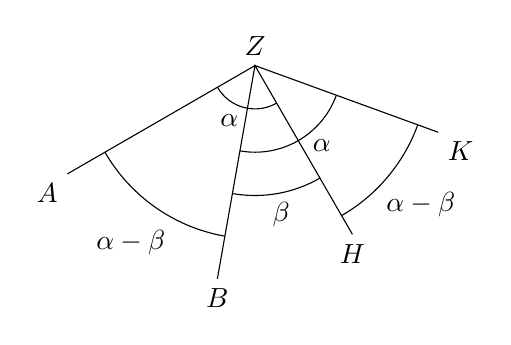
\begin{tikzpicture}[scale=.55]
\coordinate (Z) at (0,0);
\coordinate (A) at (-150:5cm);
\coordinate (B) at (-100:5cm);
\coordinate (H) at (-60:4.5cm);
\coordinate (K) at (-20:4.5cm);
\draw (A) node[below left] {$A$} -- (Z) node[above] {$Z$} -- (B) node[below] {$B$};
\draw (H) node[below] {$H$} -- (Z) -- (K) node[below right] {$K$};
\draw (-150:1cm) arc (-150:-60:1);
\draw (-100:2cm) arc (-100:-20:2);
\draw (-100:3cm) arc (-100:-60:3);
\draw (-150:4cm) arc (-150:-100:4);
\draw (-60:4cm) arc (-60:-20:4);
\node at (-115:1.4) {$\alpha$};
\node at (-50:2.4) {$\alpha$};
\node at (-80:3.5) {$\beta$};
\node at (-40:5) {$\alpha - \beta$};
\node at (-125:5) {$\alpha - \beta$};
\end{tikzpicture}
\caption{$\angle AZB=\angle HZK$}\label{f.compass-relative4}
\end{center}
\end{minipage}
\end{figure}

$\triangle ZAB\sim\triangle ZHK$, da beide gleichschenklige Dreiecke sind und wir gezeigt haben, dass sie denselben Scheitelwinkel haben. Beschriften Sie $\overline{HK}$ mit $x$. Dann:
\begin{eqnarray*}
\frac{m}{s} &=& \frac{n}{x}\\
x&=&\frac{n}{m}s\,.
\end{eqnarray*}
\end{proof}

%%%%%%%%%%%%%%%%%%%%%%%%%%%%%%%%%%%%%%%%%%%%%%%%%%%%%%%%%%%%%%%

\section{Konstruktion des Schnittpunkts von zwei Geraden}\label{s.two-lines}

\begin{theorem}
Bei zwei Linien, die die Linienabschnitte $\overline{AB}, \overline{CD}$ enthalten, ist es möglich, ihren Schnittpunkt $S$ zu konstruieren.
\end{theorem}

\begin{proof}
Seien $C',D'$ die Spiegelungen von $C,D$ um $\overline{AB}$.
Es gibt zwei Fälle, je nachdem, ob $C,D$ auf der gleichen Seite von $\overline{AB}$ oder auf verschiedenen Seiten liegen. Beschriften Sie $x=\overline{CS}, c=\overline{CC'}, d=\overline{DD'}, e=\overline{CD}$ wie in Abb.~\ref{f.compass-intersection1}, \ref{f.compass-intersection2} gezeigt. Wir berechnen den Wert von $x$ für jeden Fall.

\textit{Fall 1:}
$C,D$ liegen auf den verschiedenen Seiten von $\overline{AB}$.
$S$ liegt auf $\overline{AB}$, weil $\triangle CZS\cong \triangle C'ZS$ durch side-angle-side: $\overline{CZ}=\overline{C'Z}$, $\angle CZS=\angle C'ZS=90^\circ$ und $\overline{ZS}$ ist eine gemeinsame Seite. Daher ist $\overline{C'S}=\overline{CS}$ und ebenso $\overline{D'S}=\overline{DS}$. $\triangle CSC'\sim\triangle DSD'$ sind ähnlich, also ist $\displaystyle\frac{x}{e-x} = \displaystyle\frac{c}{d}$ und die Lösung der Gleichung ergibt $x=\displaystyle\frac{c}{c+d}e$.

\begin{figure}[ht]
\begin{center}
\begin{tikzpicture}[scale=.9]
\coordinate (A) at (-4,0);
\coordinate (B) at (2,0);
\coordinate (C) at (-3,2);
\coordinate (D) at (1,-1);
\coordinate (Cp) at (-3,-2);
\coordinate (Dp) at (1,1);
\vertex{A};
\vertex{B};
\node[below] at (A) {$A$};
\node[below] at (B) {$B$};
\node[above] at (C) {$C$};
\node[below] at (D) {$D$};
\node[below] at (Cp) {$C'$};
\node[above] at (Dp) {$D'$};
\draw[name path=ab] ($(A)!1.3!(B)$) -- ($(B)!1.3!(A)$);
\draw[name path=cd] ($(C)!1.2!(D)$) -- ($(D)!1.1!(C)$);
\path [name intersections={of=ab and cd,by={S}}];
\node[above] at (S) {$S$};
\draw (Cp) -- node[below] {$x$} (S);
\draw (S) -- node[above,xshift=-5pt] {$e\!-\!x$} (Dp);
\draw (C) -- node[above left,yshift=6pt] {$c$} (Cp);
\draw (D) -- node[above right,yshift=6pt] {$d$} (Dp);
\path (C) -- node[right,xshift=2pt] {$x$} (S);
\path (S) -- node[left,near end,xshift=-2pt] {$e\!-\!x$} (D);
\node[below left] at (C|-A) {$Z$};
\vertex{C};
\vertex{D};
\vertex{Cp};
\vertex{Dp};
\draw ($(C)!.5!(Cp)$) rectangle +(6pt,6pt);
\draw[rotate=90] ($(D)!.5!(Dp)$) rectangle +(6pt,6pt);
\end{tikzpicture}
\end{center}
\caption{Konstruktion des Schnittpunkts zweier Linien (1)}\label{f.compass-intersection1}
\end{figure}

\textit{Fall 2:}
$C,D$ liegen auf der gleichen Seite von $\overline{AB}$. $\triangle CSC'\sim\triangle DSD'$ ergibt $\displaystyle\frac{x}{x-e}=\frac{c}{d}\displaystyle$ und die Lösung der Gleichung ergibt $x=\displaystyle\frac{c}{c-d}e$.

\begin{figure}[t]
\begin{center}
\begin{tikzpicture}[scale=.9]
\coordinate (A) at (-4,0);
\coordinate (B) at (2,0);
\coordinate (C) at (-3,2);
\coordinate (D) at (-1,1);
\coordinate (Cp) at (-3,-2);
\coordinate (Dp) at (-1,-1);
\vertex{A};
\vertex{B};
\node[below] at (A) {$A$};
\node[below] at (B) {$B$};
\node[above] at (C) {$C$};
\node[above] at (D) {$D$};
\node[below] at (Cp) {$C'$};
\node[below] at (Dp) {$D'$};
\draw[name path=ab] ($(A)!1.3!(B)$) -- ($(B)!1.3!(A)$);
\draw[name path=cd] ($(C)!2.2!(D)$) -- ($(D)!1.1!(C)$);
\path [name intersections={of=ab and cd,by={S}}];
\node[above] at (S) {$S$};
\draw (Cp) -- (S);
\draw (C) -- node[above left,yshift=6pt] {$c$} (Cp);
\draw (D) -- node[above right,yshift=6pt] {$d$} (Dp);
\path (C) -- node[above] {$e$} (D);
\path (Cp) -- node[below] {$e$} (Dp);
\path (D) -- node[above right,xshift=-4pt] {$x-e$} (S);
\path (Dp) -- node[below right,xshift=-4pt] {$x-e$} (S);
\node[below left] at (C|-A) {$Z$};
\vertex{C};
\vertex{D};
\vertex{Cp};
\vertex{Dp};
\draw ($(C)!.5!(Cp)$) rectangle +(6pt,6pt);
\draw[rotate=90] ($(D)!.5!(Dp)$) rectangle +(6pt,6pt);
\end{tikzpicture}
\end{center}
\caption{Konstruktion des Schnittpunkts zweier Linien (2)}\label{f.compass-intersection2}
\end{figure}

\medskip

Konstruieren Sie die Kreise $c(C',d), c(D,e)$ und bezeichnen Sie ihren Schnittpunkt mit $H$ (Abb.~\ref{f.compass-intersection3}). Die Summe der Linienabschnitte $\overline{CC'}, \overline{C'H}$ ist $c + d$. Wir müssen zeigen, dass $H$ auf der Verlängerung von $\overline{CC'}$ liegt, so dass $\overline{CH}$ ein Liniensegment der Länge $c+d$ ist. $\overline{CH} = c - d$ für den Fall, dass $D$ auf der gleichen Seite von $\overline{AB}$ liegt wie $C$ (im Diagramm nicht dargestellt).
\begin{figure}[b]
\begin{center}
\begin{tikzpicture}[scale=.8]
\coordinate (A) at (-4,0);
\coordinate (B) at (2,0);
\coordinate (C) at (-3,2);
\coordinate (D) at (1,-1);
\coordinate (Cp) at (-3,-2);
\coordinate (Dp) at (1,1);
\vertex{A};
\vertex{B};
\node[below left] at (A) {$A$};
\node[below] at (B) {$B$};
\node[above] at (C) {$C$};
\node[below] at (D) {$D$};
\node[left] at (Cp) {$C'$};
\node[above] at (Dp) {$D'$};
\draw[name path=ab] ($(A)!1.3!(B)$) -- ($(B)!1.3!(A)$);
\draw[name path=cd] ($(C)!1.2!(D)$) -- ($(D)!1.1!(C)$);
\path [name intersections={of=ab and cd,by={S}}];
\node[above,yshift=4pt] at (S) {$S$};
\draw (Cp) -- node[below right,xshift=5pt,yshift=5pt] {$e$} (Dp);
\path (C) -- node[above left] {$c$} (Cp);
\draw[thick,dashed] (D) -- node[above right] {$d$} (Dp);
\draw[name path=circled] (D) let
  \p1 = ($ (D) - (C) $),
  \n2 = {veclen(\x1,\y1)}
in
  ++(130:\n2) arc (130:230:\n2);

\draw[name path=circlecp] (Cp) let
  \p1 = ($ (D) - (Dp) $),
  \n2 = {veclen(\x1,\y1)}
in
  ++(-180:\n2) arc (-180:0:\n2);
\path [name intersections={of=circled and circlecp,by={H}}];
\node[below left] at (H) {$H$};
\draw ($(C)!1.2!(H)$) -- (C);
\draw (H) -- node[right] {$d$} (Cp);
\draw (D) -- node[right,xshift=18pt,yshift=12pt] {$e$} (H);
\vertex{Cp};
\vertex{D};
\vertex{C};
\vertex{Dp};
\vertex{H};
\path (C) -- node[above] {$x$} (S);
\path (Cp) -- node[below] {$x$} (S);
\end{tikzpicture}
\end{center}
\caption{Konstruktion des Schnittpunkts zweier Linien (3)}\label{f.compass-intersection3}
\end{figure}

$H$ ist der Schnittpunkt von $c(C',d), c(D,e)$, also $\overline{DH}=e$, $\overline{C'H}=d$. Durch die Konstruktion $\overline{C'D'} = e$, $\overline{D'D}=d$ ist das Viereck $\overline{C'D'DH}$ also ein Parallelogramm. 

Durch Konstruktion ist $\overline{DD'}\parallel\overline{CC'}$ also $\overline{C'H}\parallel \overline{DD'}$ und somit $\overline{C'H}\parallel\overline{CC'}$. Da einer ihrer Endpunkte $C'$ ist, muss sie auf der Linie liegen, die $\overline{CC'}$ enthält. Durch Thm.~\ref{thm.add-subtract-mm} lässt sich aus den Längen $c,d,e$ ein Linienabschnitt der Länge $c+d$ konstruieren und durch Thm.~\ref{thm.compass-ratio} ein Linienabschnitt der Länge $x=\displaystyle\frac{c}{c+d}e$ konstruieren. $S$, der Schnittpunkt von $c(C',x)$ und $c(C,x)$, ist auch der Schnittpunkt von $\overline{AB}, \overline{CD}$ (Abb.~\ref{f.compass-intersection4}).
\end{proof}

\begin{figure}[t]
\begin{center}
\begin{tikzpicture}[scale=.9]
\coordinate (A) at (-4,0);
\coordinate (B) at (2,0);
\coordinate (C) at (-3,2);
\coordinate (D) at (1,-1);
\coordinate (Cp) at (-3,-2);
\coordinate (Dp) at (1,1);
\vertex{A};
\vertex{B};
\node[below left] at (A) {$A$};
\node[below] at (B) {$B$};
\node[above] at (C) {$C$};
\node[below] at (D) {$D$};
\node[left] at (Cp) {$C'$};
\node[above] at (Dp) {$D'$};
\draw[name path=ab] ($(A)!1.3!(B)$) -- ($(B)!1.3!(A)$);
\draw[name path=cd] ($(C)!1.2!(D)$) -- ($(D)!1.1!(C)$);
\path [name intersections={of=ab and cd,by={S}}];
\node[above,yshift=4pt] at (S) {$S$};
\draw (Cp) -- (Dp);
\path (C) -- node[above,yshift=4pt] {$x$} (S);
\path (Cp) -- node[below,yshift=-4pt] {$x$} (S);
\path (C) -- node[above left] {$c$} (Cp);
\draw (D) -- node[above right] {$d$} (Dp);
\draw[name path=circled] (C) let
  \p1 = ($ (S) - (C) $),
  \n2 = {veclen(\x1,\y1)}
in
  ++(-10:\n2) arc (-10:-100:\n2);

\draw[name path=circlecp] (Cp) let
  \p1 = ($ (S) - (C) $),
  \n2 = {veclen(\x1,\y1)}
in
  ++(100:\n2) arc (100:0:\n2);
\draw (Cp) -- (C);
\vertex{C};
\vertex{Cp};
\vertex{D};
\vertex{Dp};
\end{tikzpicture}
\end{center}
\caption{Konstruktion des Schnittpunkts zweier Linien (4)}\label{f.compass-intersection4}
\end{figure}

%%%%%%%%%%%%%%%%%%%%%%%%%%%%%%%%%%%%%%%%%%%%%%%%%%%%%%%%%%%%%%%

\section{Konstruktion des Schnittpunkts einer Linie und eines Kreises}\label{s.line-circle}

\begin{theorem}
Bei einem Kreis $k=C(M,r)$ und einer Linie $l$ kann man die Schnittpunkte von $k$ und $l$ konstruieren.
\end{theorem}

\begin{proof}
Konstruieren Sie $M'$, sei die Spiegelung von $M$ um $l$ und konstruieren Sie den Kreis $k'=c(M',r)$. Da $\triangle MYM'\cong\triangle MXM'$ ist, sind $X,Y$, die Schnittpunkte von $k,k'$, die Schnittpunkte von $l$ und $k$ (Abb.~\ref{f.compass-circle4}).
\begin{figure}[t]
\begin{center}
\begin{tikzpicture}[scale=.5]
\coordinate (A) at (-7,0);
\coordinate (B) at (8,0);
\coordinate (M) at (0,-2);
\coordinate (Mp) at (0,2);
\node[below left] at (M) {$M$};
\node[above left] at (Mp) {$M'$};
\draw[name path=c1] (M) circle[radius=3cm];
\draw[name path=c2] (Mp) circle[radius=3cm];
\draw[name path=ab] ($(A)!1.2!(B)$) --
  node[above,very near end] {$l$} ($(B)!1.2!(A)$);
\path [name intersections={of=c1 and c2,by={S1,S2}}];
\path[name path=radius1] (M) -- ++(15:4cm);
\path [name intersections={of=c1 and radius1,by={R1}}];
\draw (M) -- node[below] {$r$} (R1);
\path[name path=radius2] (Mp) -- ++(40:4cm);
\path [name intersections={of=c2 and radius2,by={R2}}];
\draw (Mp) -- node[above] {$r$} (R2);
\draw (Mp) -- (M) -- (S1) -- (Mp) -- (S2) -- (M);
\node[right,xshift=6pt,yshift=6pt] at (S1) {$X$};
\node[left,xshift=-6pt,yshift=6pt] at (S2) {$Y$};
\draw (0,0) rectangle +(10pt,10pt);
\node at (-3.5,-3) {$k$};
\node at (-3.5,3) {$k'$};
\end{tikzpicture}
\end{center}
\caption{Konstruktion des Schnittpunkts zwischen einer Linie und einem Kreis (1)}\label{f.compass-circle4}
\end{figure}

Diese Konstruktion kann nicht durchgeführt werden, wenn $M$ auf der Linie $l$ liegt. In diesem Fall ist ein beliebiger Punkt $A$ auf $l$ zu wählen, der mehr als $r$ von $M$ entfernt ist. Mit Thm~\ref{thm.add-subtract-mm} verkürzt und verlängert man $\overline{AM}$ um $r$. $X,Y$, die Endpunkte dieser Segmente, sind die Schnittpunkte von $k$ und $l$ (Abb.~\ref{f.compass-circle5}).
\end{proof}

\begin{figure}[b]
\begin{center}
\begin{tikzpicture}[scale=.5]
\coordinate (A) at (-7,0);
\coordinate (B) at (8,0);
\coordinate (M) at (0,0);
\vertex{M};
\vertex{A};
\node[below] at (A) {$A$};
\node[below left] at (M) {$M$};
\draw[name path=c1] (M) circle[radius=3cm];
\draw[name path=ab] ($(A)!1.2!(B)$) -- 
  node[above,very near end] {$l$} ($(B)!1.2!(A)$);
\path[name path=radius1] (M) -- ++(50:4cm);
\path [name intersections={of=c1 and radius1,by={R1}}];
\draw (M) -- node[above] {$r$} (R1);
\path [name intersections={of=c1 and ab,by={S1,S2}}];
\node[above right] at (S1) {$X$};
\node[above left] at (S2) {$Y$};
\path (M) -- node[below,xshift=4pt] {$\overline{AM}+r$} (S1);
\path (A) -- node[below] {$\overline{AM}-r$} (S2);
\node at (-2.5,2.5) {$k$};
\end{tikzpicture}
\end{center}
\caption{Konstruktion des Schnittpunkts zwischen einer Linie und einem Kreis (2)}\label{f.compass-circle5}
\end{figure}


\subsection*{Was ist die Überraschung?}

Wenn man etwas über Konstruktionen mit einem Lineal und einem Zirkel lernt, ist es offensichtlich, dass beide Werkzeuge notwendig sind. Daher war es eine ziemliche Überraschung, herauszufinden, dass ein Zirkel ausreicht. Der Beweis ist ziemlich lang, also werden wir das Lineal nicht zu Hause lassen, aber das Theorem zeigt, dass wir nicht davon ausgehen sollten, dass es keine Alternativen zu bekannten mathematischen Konzepten gibt.

\subsection*{Quellen}

Dieses Kapitel basiert auf dem Problem $33$ aus \cite{dorrie1}, das von Michael Woltermann \cite{dorrie2} überarbeitet wurde. Ein zusätzlicher Beweis ist in \cite{mm} zu finden.
